%!TEX root = ../main.tex

\chapter{Preliminaries\label{chap:preliminaries}}
\alertwarning{Under construction}

\section{Radioactivity}


\section{Radioactive decay}
Radioactive decay is the process by which an unstable atomic nucleus loses energy by radiation. 


\section{Health risk}


\section{Properties of gamma radiation}
  \subsection{Activity of the source}
  \subsection{Inverse square law}% %%{
The important property of ionizing radiation is that the intensity of the radiation decreases with the inverse square law.
In other words, the intensity at a given point is proportional to $\frac{1}{d^{2}}$, where $d$ is the distance from the source.
  \begin{figure}[!h]
    \centering
      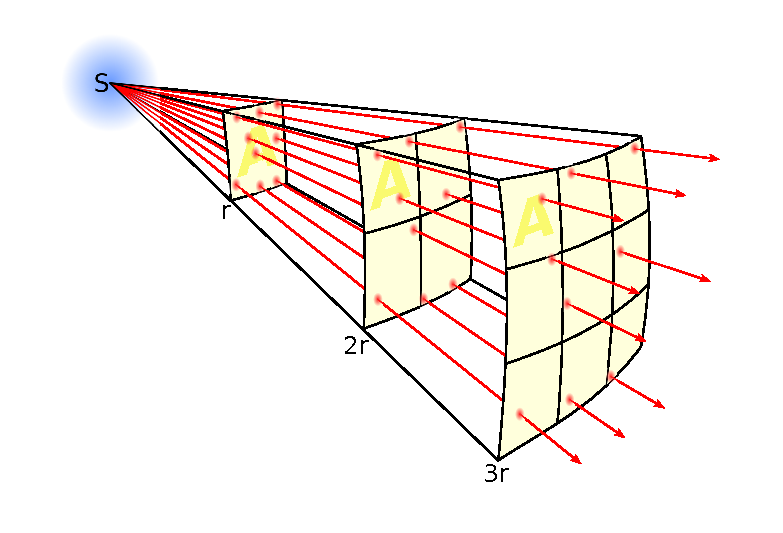
\includegraphics[width=0.2\textwidth]{./fig/photos/Inverse_square_law.eps}
      \label{fig:isl}
    \caption{An illustration of inverse square law for radioactive decay, source \protect \footnote{By Borb, CC BY-SA 3.0, https://commons.wikimedia.org/w/index.php?curid=3816716i}}
  \end{figure}

% %%}

\subsection{attenuationnnn}

\section{Interaction with matter}
\section{photoelectric absorbtion}
\section{Compton scattering}

\section{pair production}
\subsection{Klein-Nishina}
\section{Interaction with matter}
alpha, beta, gamma

\section{Measuring radioactivity}


\section{Interaction with matter}

\begin{figure}[!h]% %%{
  \centering
  \subfloat[\centering Cross-section for photon interactions in Silicon in the MeV range. The four dominating interaction mechanisms are photo effect, Compton scattering, pair creation and Rayleigh scattering. Source: \cite{zoglauer}] {
    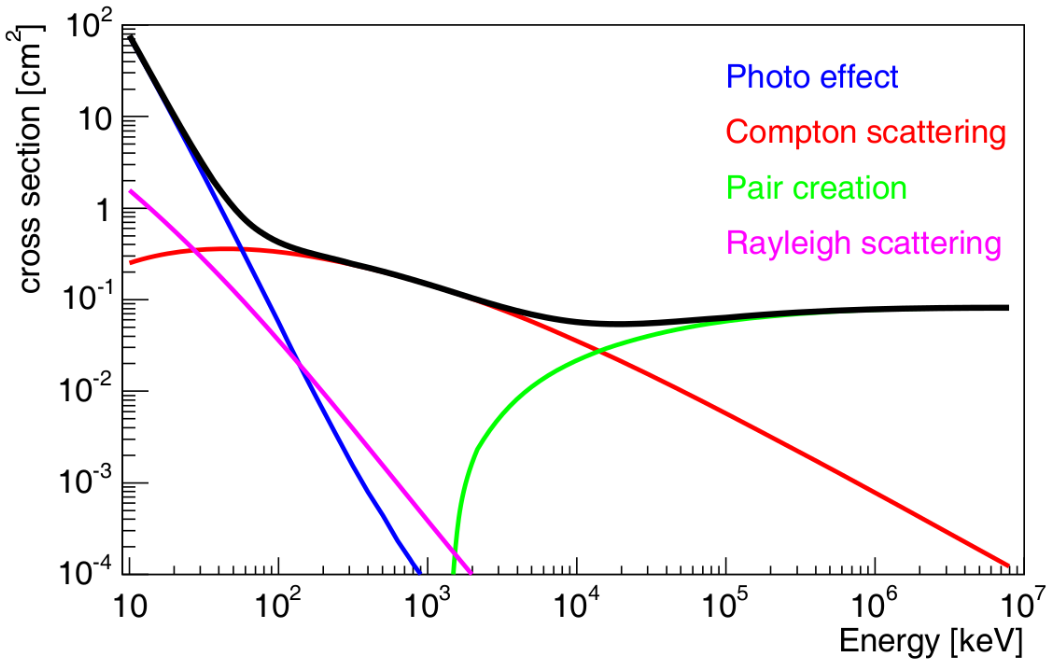
\includegraphics[width=0.45\textwidth]{./fig/photos/cross_stat.png}
    \label{fig:dis2}
  }
  \subfloat[\centering Cross section for compton scattering. Source: \cite{zoglauer}] {

    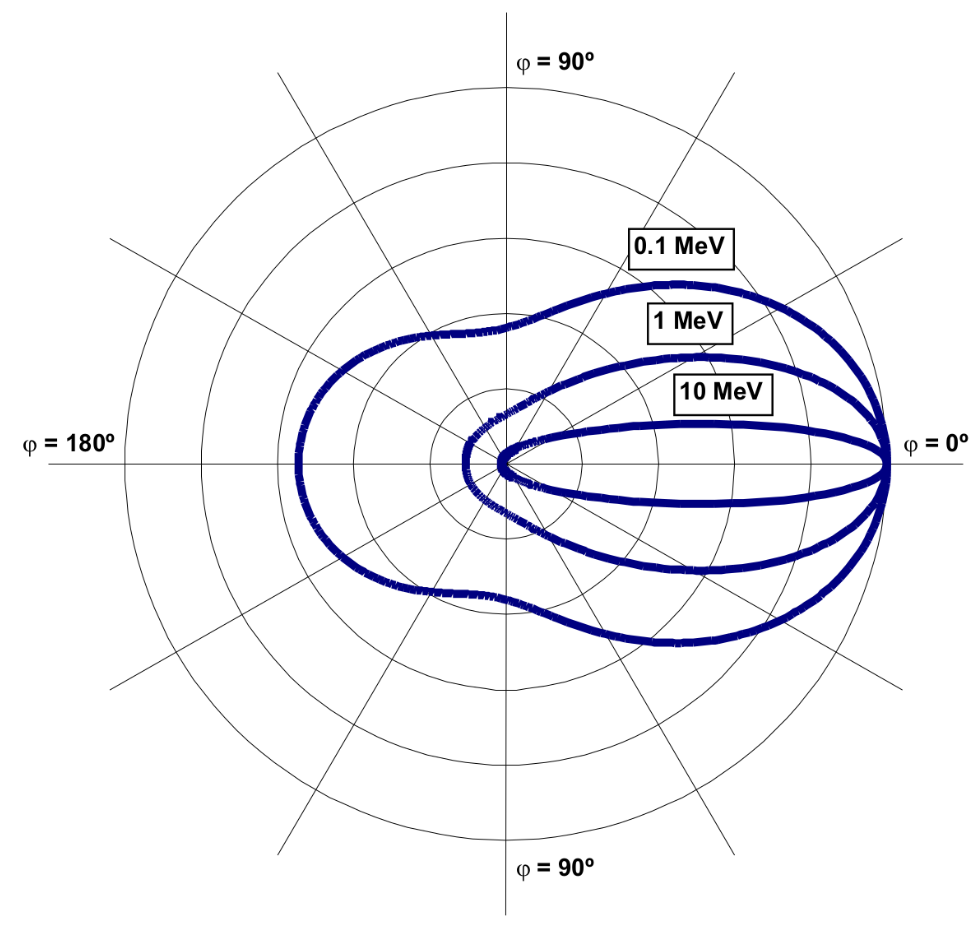
\includegraphics[width=0.45\textwidth]{./fig/photos/cross_section.png}
    \label{fig:dis1}
  }
  \caption{TODO}
  \label{fig:xxx}
\end{figure}% %%}

\subsection{Compton scattering}% %%{

During the Compton scattering, the $\gamma$ photon interacts with an electron loosely bound to the nucleus.
The photon with initial energy $E_{0}$ transfers part of it to the electron.



\begin{figure}[!h]
    \centering
    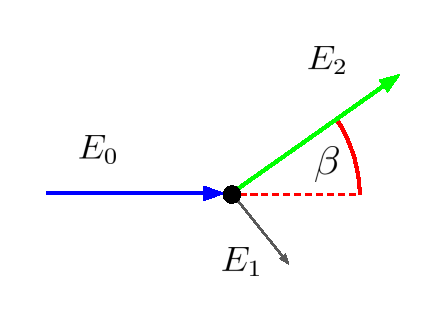
\includegraphics[width=0.3\textwidth]{./fig/photos/compton_simple.eps}
    \caption{An illustration of the Compton scattering. The incident $\gamma$ photon with energy $E_{0}$ (blue) undergoes the Compton scattering. As a result of the interaction, the lower energetic photon (green) with energy $E_{2}$ is emitted under angle $\beta$. Part of the energy ($E_{1}$) is transferred to a bi-product of the interaction- the electron (grey).}
    \label{fig:scattering}
\end{figure}
The probability that a photon with an energy $E_{0}$ undergoes a Compton scattering through an angle $\beta$ is described by the Klein-Nishina formula
\begin{equation}
  K(\beta, E_{0}) = \frac{r_{e}^{2}}{2} \left( \frac{E_{2}}{E_{0}}  \right)^{2} \left(  \frac{E_{2}}{E_{0}} + \frac{E_{0}}{E_{2}} - \mathrm{sin}^{2}(\beta)  \right)
  \label{eq:klein_nishina}
\end{equation}


According to Compton \cite{compton}, the relation of particle energies and scattering angle $\beta$ is

\begin{equation}
E_{2} = \frac{E_{0}}{  1 + (E_{0} / m_{e}c^{2}) (1 - \mathrm{cos} \beta)},
\end{equation}
where $E_{0}$ is the initial energy of the incoming photon, $E_{2}$ is the energy of scattered photon,  $m_{e}$ is the electron rest mass and $c$ is the speed of light in vacuum. 


% %%}

\subsection{Compton Camera}% %%{
The Compton camera is typically composed of two detectors: scatterer and absorber.
The incident photon with energy $E_{0}$ first interacts with the scatterer at position $X_{1}$ in form of Compton scattering.
A bi-product of the interaction (electron with energy $E_{1}$) is immediately captured by the scatterer and its position $X_{1}$ and energy are recorded.
As a result of the interaction, lower energetic photon with energy $E_{2}$ is scattered under (Compton) angle $\beta$.
The scattered photon then interacts in form of \ac{PE} with the absorber.
The absorbed energy $E_{2}$ and the position of the interaction $X_{2}$ are measured and recorded.

The scattering angle $\beta$ can be reconstructed (following \cite{baca2021gamma}) as:
\begin{equation}
  %\beta = \mathrm{arccos} \left (  1-\frac{m_{e}c^{2}E_{2}}{E_{0} (E_{0} - E_{2})} \right )
  \beta = \mathrm{cos}^{-1} 
  \underset{B}{\underbrace{
  \left ( 1+m_{e}c^{2} \left( \frac{1}{E_{1}+E_{0}} - \frac{1}{E_{0}}\right )  \right )
  }},
    \label{eq:compton_beta_formula}
\end{equation}
assuming that $0<B<1$.
Since the Compton scattering is a symmetrical phenomena,  the set of possible directions of incoming particle forms a surface of a cone.
Such conical surface (denoted as Compton cone) is parametrized by the cone axis $a$ (which is a straight line connecting the positions of intersections $X_{1}$ and $X_{2}$), Compton scattering angle $\beta$ and origin of the cone $X_{1}$.
The geometry is illustrated in figure \ref{fig:compton_camera_geometry}.

  \begin{figure}[!h]
    \centering
      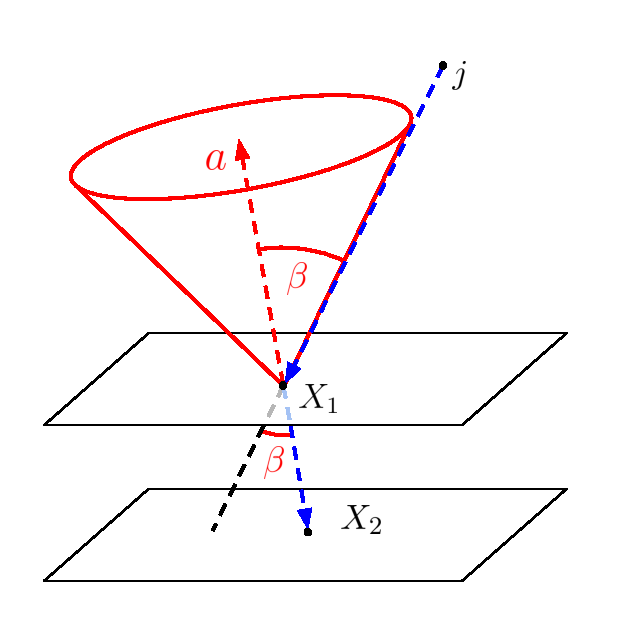
\includegraphics[width=0.4\textwidth]{./fig/photos/compton_camera_modelll.eps}
      \caption{Geometry for two-layer Compton camera. The $\gamma$ particle emitted at position $j$ interacts with the first layer of the sensor (scatterer) at position $X_{1}$. A lower energetic photon is scattered under angle $\beta$ and absorbed by the second layer of the detector (absorber) at position $X_{2}$. The reconstructed Compton cone is parametrized by angle $\beta$, axis vector $a$ and origin of the cone $X_{1}$.}
      \label{fig:compton_camera_geometry}
  \end{figure}

% %%}


\section{The MiniPIX TPX3 detector} 
The MiniPIX TPX3 detector\footnote{produced by \textit{Advacam}, https://advacam.com/camera/minipix-tpx3} is a miniature version Timepix3 detector \cite{timepix3}.
It belongs to the class of semiconductor pixel detectors.
The body of the \ac{pix} sensor is made of a compact block of Cadmium telluride (CdTe) semiconductor material with dimensions $14 \times 14 \times 2 \ \si{\milli\meter}$.
Although it has only one detection layer, it can be still used as a Compton camera.

As described in \cite{baca2021gamma} and \cite{baca2019timepix}, the incoming ionizing radiation interacts with the matter of the sensor and separates electrons from the CdTe material.
The newly created electrons are accelerated by a $\SI{450}\volt$ electric potential towards one facet of the sensor, where Timepix3 pixel detector is located.
The resolution of pixel detector is $256 \times 256\ \mathrm{px}$, each pixel being $55\ \si{\micro\meter}$ large.
The pixel detector can deduce the energy as well as the type of the absorbed ionizing particle.
Given the measured times of arrival, the coinciding products of Compton scattering might be paired together.
The figure \ref{fig:minipix} depicts the geometry of the \ac{pix} sensor.
The 2D coordinates $\mathbf{\hat{c}}_{x}$,$\mathbf{\hat{c}}_{x}$ (see figure \ref{fig:minipix}) of the interaction are determined by the position of corresponding pixels
The $\mathbf{\hat{c}}_{z}$ coordinate (the depth of interaction in the CdTe block) is unknown.
However, the relative depth position of two coinciding events might be deduced from the times of arrival of the two interactions were captured by the pixel detector.
Because of that, the \ac{pix} detector might be used as a Compton camera.
More technical details related to the sensor operation are provided in \cite{baca2019timepix}.

The \ac{pix} detector has multiple advantages.
It is very compact and lightweight (the size of the whole \ac{pix} sensor is only $80 \times 21 \times 14 \ \si{\milli\meter}$ and it weights $\SI{44}{\gram}$), therefore it can be carried onboard a small \ac{UAV}.
It can report the recorded intersections almost in real time, which allows the to use it for an active strategy, where autonomous \ac{UAV}s react according to the measurements acquired during the flight.

\begin{figure}[!h]
    \centering
    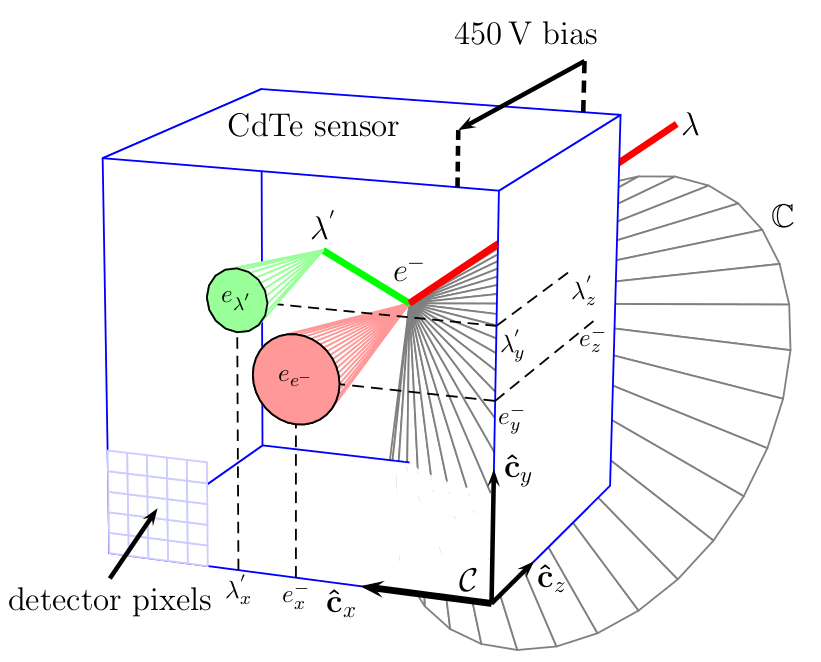
\includegraphics[width=0.7\textwidth]{./fig/photos/minipix.png}
    \caption{An illustration of the detection process inside the MiniPIX TPX3 sensor. Source: \cite{baca2021gamma}}
    \label{fig:minipix}
\end{figure}



\subsection{semiconductior detectors}
\subsection{Minipix TPX3}

\section{ROS}
\subsection{Rosbag}
\subsection{architecture}
\subsection{Nodes, Messages and Services}

%%%%%%%%%%%%%%%%%%%%%%%%
%%%%%%%%%%%%%%%%%%%%%%%%%%
%%%%%%%%%%%%%%%%%%%%%%%
%%%%%%%%%%%%%%%%%%%%%%%%%%%%
%%%%%%%%%%%%%%%%%%%%%%%%%%
%%%%%%%%%%%%%%%%%%%%%%%%
\alerterror{Old}
\section{Radioactive decay}
Radioactive decay is a process where an unstable atomic nucleus transforms into a lower-energy state.
During this process, it loses energy by radiation.
There are three main types of such radiation - alpha, beta and gamma.
Whereas alpha particles can be stopped by a sheet of paper and beta particles by aluminium shielding, gamma particles can be blocked only using a thick block of lead or a massive concrete wall.
Moreover, highly energetic gamma rays have a negative effect on the human body, causing damage on a cellular level.
Being exposed to such radiation poses a risk of severe health problems or death.

\section{Some properties of $\gamma$ radiation}
\subsection{Inverse square law}
\subsection{Interaction with matter}

The quantity of emitted particles ("strength" of the source) is expressed in Becquerels.
It is a SI unit defined as the number of emitted particles per second.

\section{Interaction with matter}
As the gamma particle passes through matter, there are three possible effects that might happen:
\textbf{the photoelectric effect}, \textbf{Compton scattering} and \textbf{pair production}.

\textbf{The photoelectric effect} is typical at low energies of gamma rays. A photon undergoes an interaction with an electron that is bound in an atom. The incident photon completely disappears in this interaction. A product of this interaction is a photon.
\textbf{The Compton effect} is typical for mid-energetic gamma rays. In this process, an incident gamma photon loses energy to an atomic electron. A new lower energetic photon is emitted in a different direction (hence the frequently used term "Compton scattering").
\textbf{Pair production} is typical for high-energetic gamma rays. It is a process in which a photon of sufficient energy is converted into an electron and a positron.

The Compton effect (published in 1923 \cite{}) describes the way how a (gamma or X-ray) photon interacts with a static electron. An incident photon with wavelength $\lambda$ losses some energy to the electron. A new lower energetic photon with wavelength $\lambda^{\prime}$ is emitted under angle $\beta$. Thanks to the law of conservation of energy and momentum, Compton derived the following equation
\begin{equation}
    \lambda^{\prime} = \lambda + \frac{h}{m_{e}c}(1-\mathrm{cos} \beta),
\end{equation}
where $\lambda$ is the wavelength of the incident photon, $\lambda^{\prime}$ is the wavelength of the emitted photon, $h$ is the Planck constant, $m_{e}$ is the electron rest mass, $c$ is the speed of light and $\beta$ is the scattering angle.

\begin{figure}[!h]
    \centering
    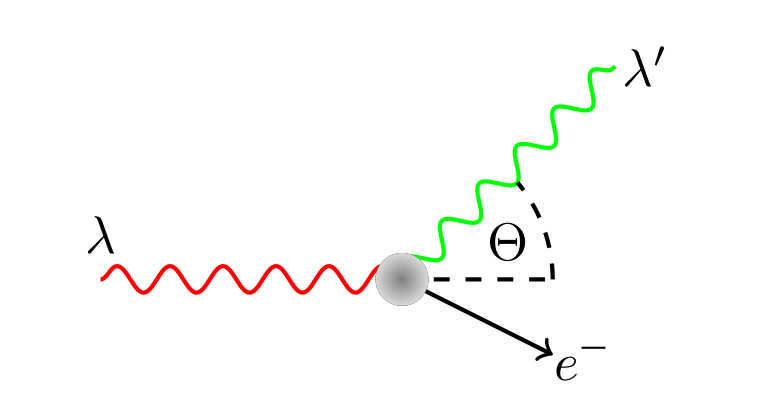
\includegraphics[width=0.3\textwidth]{./fig/photos/scattering.png}
    \label{fig:scattering}
    \caption{An illustration of Compton scattering. The incident photon interacts with the static electron. As a result, a new lower energetic photon is emitted in a direction changed by $\beta$ as part of its energy is transferred to electron $e^{-}$. Source: \cite{baca2021gamma}}
\end{figure}


\subsection{Klein Nishina formula}
TODO

\subsection{Compton effect}
TODO


\section{Compton camera}
This effect is the fundamental principle in a sensor called a Compton camera. 
The sensor is typically composed of two main components: the scatterer and the absorber. 
The incident photon first interacts with the scatterer, where the lower energetic photon is emitted under angle $\beta$ (thanks to the Compton effect). 
Since it is more common to measure energies instead of wavelength, we can rewrite the Compton formula as
\begin{equation}
E_{\lambda^{\prime}} = \frac{E_{\lambda}}{  1 + (E_{\lambda} / m_{e}c^{2}) (1 - \mathrm{cos} \beta)},
\end{equation}
where $E_{\lambda}$ is the energy of the incoming photon from the source, $E_{\lambda^{\prime}}$ is the energy of the scattered photon.  
The bi-product of the interaction (electron $e_{e^{-}}$) is immediately measured in the scatterer, and its position is recorded.
Then, the scattered lower energetic photon interacts with the second layer of the sensor - the absorber. 
The photoelectric effect is witnessed while measuring the product of it - the energy of the electron $e_{\lambda^{prime}}$ and its position on the absorber.

Now we can express the scattering angle $\beta$ as
\begin{equation}
    \beta = \mathrm{arccos} \left (  1-\frac{m_{e}c^{2}E_{\lambda^{\prime}}}{E_{\lambda} (E_{\lambda} - E_{\lambda^{\prime}})} \right )
    %\label{eq:compton_beta_formula}
\end{equation}

Given the measurements on the scatterer and absorber and computed scattering angle $\beta$ using the equation \ref{eq:theta} (using known energy of the incoming photon $E_{\lambda}$), we can reconstruct a set of possible directions from where the original photon arrived. Since the Compton effect is symmetrical, the set of possible directions towards the source of ionizing radiation forms a surface of a cone.



\subsection{MiniPIX TPX3 sensor}
The sensor used in this work is a small CdTe event-based camera that is capable of witnessing the interactions between gamma photons and the matter of the sensor and reporting them in real time.
Unlike the traditional model of the Compton camera mentioned before, this is a single-stack detector.
In other words, there is no distinction between the scatterer and the absorber and all the measurable interactions are happening in one 14x14x2 mm block of CdTe semiconductor material.
The sensor is capable of measuring a 3D position of the interactions (and distinguishing its type) inside the detector with nanosecond resolution. 
All these features open the possibility of using it in Compton camera mode.
Technical details of the sensor are described in \cite{baca2021gamma} and \cite{baca2019timepix}.
The biggest advantage of this sensor is its small size, low weight and low power consumption.
Thanks to that, we can use this sensor on board a small UAV. 


\section{Cs137}

\section{ROS}

\section{MRS UAV system}

